\usetikzlibrary{arrows.meta,patterns}
\begin{frame}{appending}
    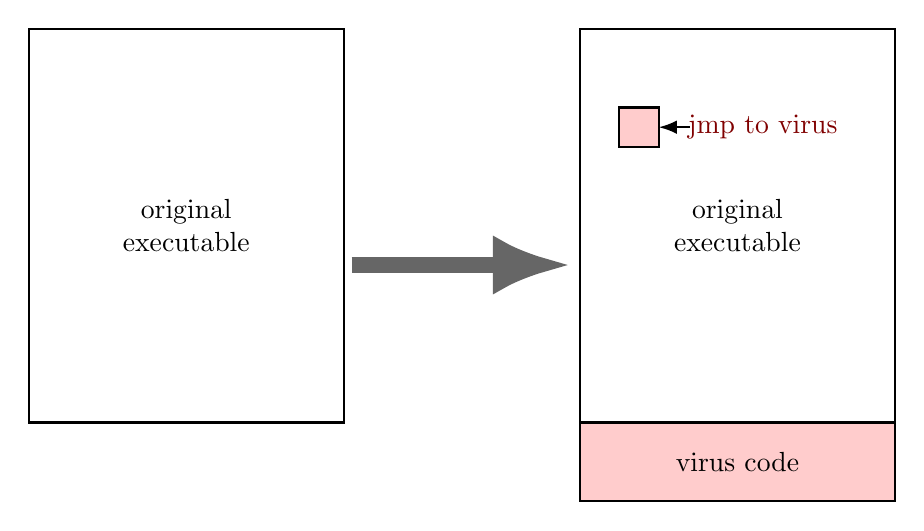
\begin{tikzpicture}
    \draw[thick] (0, 0) rectangle (4, -5) node[midway,align=center] {original\\executable};
    \draw[line width=2mm,-Latex,black!60] (4.1, -3) -- (6.9, -3);
    \begin{scope}[xshift=7cm]
    \draw[thick] (0, 0) rectangle (4, -5) node[midway,align=center] {original\\executable};
    \draw[fill=red!20,thick] (0, -5) rectangle (4, -6)
        node[midway,align=center] {virus code};
    \draw[fill=red!20,thick] (0.5, -1) rectangle (1, -1.5);
    \node[anchor=west,red!50!black] at (1.25, -1.25) {jmp to virus};
    \draw[thick,Latex-] (1, -1.25) -- (1.4, -1.25);
    \end{scope}
    \end{tikzpicture}
\end{frame}

\begin{frame}{appending and executable formats}
    \begin{itemize}
    \item COM files are very simple --- no metadata
    \item modern executable formats have length information to update:
    \vspace{.5cm}
    \item option 1: add segment (ELF LOAD) to program header
        \begin{itemize}
        \item (often a little extra space after program header, due to page-alignment)
        \end{itemize}
    \item option 2: update last segment of program header
        \begin{itemize}
        \item change its size
        \item make it executable if it isn't (and often not --- often data)
        \end{itemize}
    \end{itemize}
\end{frame}
